\subsection*{Ejercicio 3}

\ejercicio{Junto con este guión se le ha suministrado un fichero
  \textit{ejercicio-desc.cpp}. En él se ha implementado un
  algoritmo. Se pide que:}

\begin{enumerate}
\item \ejercicio{Explique qué hace este algoritmo.} Se trata de un
  algoritmo de busqueda binaria. Se parte de un vector ordenado y se
  eligen dos variables que representan los extremos del vector. Una
  vez fijadas las variables \textit{sup} e \textit{inf} seleccionamos
  la posición que está en el \textit{'centro'} respecto a ambas. Si
  coincide con lo que buscamos hemos terminado, si es más granda
  cambiamos el extremo infererior a este valor del \textit{'centro'} y
  si es menor cambiamos el extremo superior.

\item \ejercicio{Calcule su eficiencia teórica.} La complejidad teórica es $log_2(n)$ ya que fuera del bucle
  \textit{while} todo tiene complejidad $O(1)$ y dentro, en cada
  iteración, reducimos la condición en un orden de dos. Por tanto el
  algoritmo tiene la mayor de las complejidades, $log_2(n)$.

\item \ejercicio{Calcule su eficiencia empírica.}

\begin{figure}[H]
  \centering
  \caption{Eficiencia empírica}
  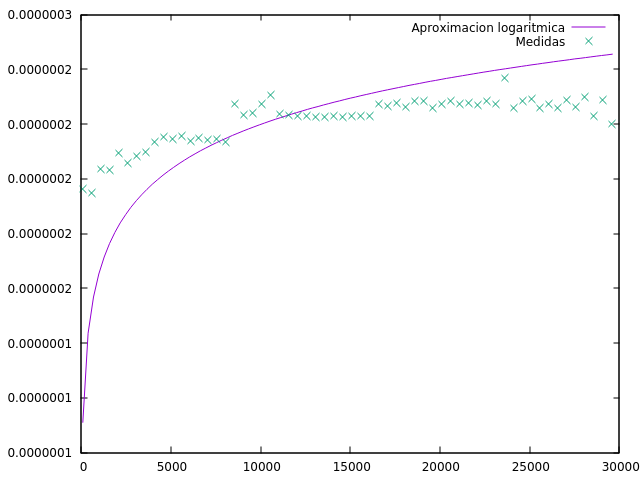
\includegraphics[width=0.8\textwidth]{ejer3/comparacion.png}
\end{figure}

\begin{flushleft}
  Se presentó el inconveniente de que las medidas en tiempo eran muy
  pequeñas y por lo tanto muchos datos habían tomado como tiempo de
  ejecución el valor 0. Para solucionar este problema se procedió a
  calcular la media aritmética del tiempo empleado en ejecutar la
  función con los mismos datos un número determinado de veces.
\end{flushleft}

\begin{flushleft}
  Por algún motivo la nube de puntos obtenida no se ajusta a una
  función logarítimica de manera óptima. Se ha probado a tomar más
  datos y a cambiar los intervalos en los que se toma pero no se
  obtuvieron medidas mejores.
\end{flushleft}

\end{enumerate}
